\documentclass{beamer}
\usepackage{listings}
\lstset{
%language=C,
frame=single, 
breaklines=true,
columns=fullflexible
}
\usepackage{blkarray}
\usepackage{subcaption}
\usepackage{url}
\usepackage{algorithm}
\usepackage{algorithmic}
\usepackage{arevmath}     % For math symbols
%\usepackage{algpseudocode}
\usepackage{optidef}
\usepackage{graphicx}
\usepackage{tikz}
\usepackage{tkz-euclide} % loads  TikZ and tkz-base
%\usetkzobj{all}
\usetikzlibrary{calc,math}
\usepackage{float}
\newcommand\norm[1]{\left\lVert#1\right\rVert}
\renewcommand{\vec}[1]{\mathbf{#1}}
\usepackage[export]{adjustbox}
\usepackage[utf8]{inputenc}
\usepackage{amsmath}
\usepackage{tikz}
\usepackage{hyperref}
\usepackage{mathtools, nccmath}


\usepackage{bm}
\hypersetup{
    colorlinks = true,
    linkbordercolor = {white},
    linkcolor={red},
    citecolor={green},
    filecolor={blue},
	menucolor={red},
	runcolor={cyan},
	urlcolor={blue},
	breaklinks=true
}
\usetikzlibrary{automata, positioning}
\usetheme{Boadilla}
\providecommand{\pr}[1]{\ensuremath{\Pr\left(#1\right)}}
\providecommand{\mbf}{\mathbf}
\providecommand{\qfunc}[1]{\ensuremath{Q\left(#1\right)}}
\providecommand{\sbrak}[1]{\ensuremath{{}\left[#1\right]}}
\providecommand{\lsbrak}[1]{\ensuremath{{}\left[#1\right.}}
\providecommand{\rsbrak}[1]{\ensuremath{{}\left.#1\right]}}
\providecommand{\brak}[1]{\ensuremath{\left(#1\right)}}
\providecommand{\lbrak}[1]{\ensuremath{\left(#1\right.}}
\providecommand{\rbrak}[1]{\ensuremath{\left.#1\right)}}
\providecommand{\cbrak}[1]{\ensuremath{\left\{#1\right\}}}
\providecommand{\lcbrak}[1]{\ensuremath{\left\{#1\right.}}
\providecommand{\rcbrak}[1]{\ensuremath{\left.#1\right\}}}
\providecommand{\abs}[1]{\vert#1\vert}
\newcommand{\comb}[2]{{}^{#1}\mathrm{C}_{#2}}
\graphicspath{ {./figs/} }
\DeclarePairedDelimiter{\nint}\lfloor\rceil
\title{Presentation on 'Energy Efficient Data Collection in UAV Enabled Wireless Sensor Networks'}
\author{Jatin Tarachandani}
\date{CS20BTECH11021}
\begin{document}

\begin{frame}
\titlepage
\end{frame}
\begin{frame}{}
\begin{block}{Authors}
\begin{itemize}
    \item Cheng Zhan
    \item Yong Zeng
    \item Rui Zhang
\end{itemize}

\end{block}
\begin{block}{Abstract}
\begin{itemize}
\item In wireless sensor networks, utilizing the unmanned
aerial vehicle (UAV) as a mobile data collector for the sensor
nodes (SNs) is an energy-efficient technique to prolong the network lifetime.
\item A method is proposed to jointly optimize the SNs’ wakeup schedule and UAV’s trajectory to minimize the maximum
energy consumption of all SNs, while ensuring that the required
amount of data is collected reliably from each SN.
\end{itemize}
\end{block}
\end{frame}
\begin{frame}{Introduction}
\begin{enumerate}
   \item Wireless sensor networks consist of multiple sensor nodes(SNs) which are generally powered by limited energy sources that are difficult to recharge. Therefore, efficient data collection is useful to prolong the lifetime of SNs. 
   \item Using a UAV to collect data from these SNs is a possible method of energy efficient data collection, since it can collect the data from SNs by manually passing near to them, reducing the transmission distance and thus also saving transmission power.
   \item Another useful technique is the use of sleep and wake up cycles for SNs so they are only transmitting when the UAV sends them a waking beacon signal at the shortest distance from them.
   \end{enumerate}
\end{frame}

\begin{frame}{Concepts}
    \begin{block}{Block fading}
    It is a type of fading (attenuation variation of a signal) in which the fading process is roughly constant for short intervals, called blocks.
    
    \end{block}
    \begin{block}{Mixed Integer Non-Convex Optimization}
    \begin{enumerate}
        \item Mixed Integer: Some elements of the constraints are constrained to assume integer values only.
        \item Non-Convex: The objective or any of the constraints may be non convex, i.e the line segment joining 2 points in the feasible region may or may not lie completely within the region. 
    \end{enumerate}
    \end{block}
\end{frame}
\begin{frame}{Terms and Notation}
\begin{itemize}
    \item We consider K SNs, each denoted by $u_k, 1 \leq k \leq K$, located at $w_k$  $\epsilon$  $R^2$, each generates $S_k$ bits of data.
    \item UAV: total flight time $T$, constant altitude $H$, max. speed $V_{max}$, initial and final coordinates denoted by $q_0$ and $q_f$. 
    \item We split $T$ into $M$ discrete time slots of $\delta_t$ duration, such that during one time slot the UAV's position is approximately unchanged w.r.t the SNs even at max speed. 
    \item Hence, we denote the UAV's trajectory as $q[m], 1 \leq m \leq M$ with $q[m]\equiv q(m \delta_t)$, representing UAV position at time slot m.
    \item We assume that only one SN can be awake at a time. We take $x_k[m]$ as the wake up schedule variable, with $x_k[m]=1$ implying the $k$'th SN is awake at time slot $m$, and $x_k[m]=0$ implying the $k$'th SN is asleep at time slot $m$.
\end{itemize}
\end{frame}
\begin{frame}{Assumptions about fading channel}
 We assume that the SN to UAV link is a quasi static block fading channel, i.e within each fading block the signal is constant and it may change between blocks. 
 The duration of each fading block is typically much smaller than $\delta_t$. Therefore we consider $L$ fading blocks in a single time slot, with $L>1$.
\end{frame}
\begin{frame}
\begin{block}{}
The channel coefficient between the SN and UAV at the $l^{th} [1 \leq l \leq L]$ fading block of time slot $m$ is given by:
\begin{align}
    h_k[m,l]=\sqrt{\beta_k[m]}\rho_k[m,l]\label{chan co}
\end{align}
\begin{itemize}
    \item $\rho_k[m,l]$ : a small scale fading coefficient
    \item $\beta_k[m]$ : fading coefficient depending on distance between SN and UAV.
\end{itemize}
\end{block}
\begin{block}{Calculation of $\beta_k[m]$}
\begin{align}
    \beta_k[m]=\frac{\beta_0}{\brak{H^2+||q[m]-w_k||^2}^\frac{\alpha}{2}}\label{beta}
\end{align}
where $\beta_0$ is the reference power gain at 1m distance, and $\alpha \geq 2$ is the path loss exponent. 
\end{block}
\end{frame}

\begin{frame}
In \eqref{chan co} and subsequently, WLOG, we take $\rho_k[m,l]$ as i.i.d random variables with the CDF of $\rho_k[m,l]^2$ given by $F\brak{\cdot}$. Also,
\begin{equation}
    E\brak{|\rho_k[m,l]|^2}=1.
\end{equation}
\begin{block}{}
The achievable transmission rate $C_k$ is obtained by
\begin{equation}
    C_k[m,l]=\log_2\brak{1+\frac{|h_k[m,l]|^2 P_k}{\sigma^2 \Gamma}}\label{Ck}
\end{equation}
where 
\begin{itemize}
    \item $\sigma^2$ is noise power
    \item$\Gamma>1$ is the SNR gap between practical modulation scheme and theoretical Gaussian signalling.
    \item $P_k$ is the transmission power of the $k$'th SN.
\end{itemize}
\end{block}
\end{frame}
\begin{frame}
We want to design the transmission rate of the awake SN $R_k[m]$ such that the outage probability $p_k[m,l]$ does not exceed a certain tolerance $\epsilon$.

\begin{align}
    p_k[m,l]&=\pr{C_k[m,l]<R_k[m]}\\\label{outagepro}
    &=\pr{\abs{\rho_k[m, l]}^2 <\frac{\sigma^2\Gamma \brak{2^{R_k[m]}-1}}{\beta_k[m]P_k}}\\
    &=F\brak{\frac{\sigma^2\Gamma \brak{2^{R_k[m]}-1}}{\beta_k[m]P_k}}\\
    &\equiv p_k^{out}[m]
\end{align}
\begin{block}{}
Now we set $p_k^{out}[m]$ to $\epsilon$ to find $R_k[m]$ such that the target amount of data can be collected reliably from each SN. 
     
 From \eqref{beta} and \eqref{outagepro}, 
\begin{align}
R_k[m]=\log_2\brak{1+\frac{F^{-1}\brak{\epsilon}P_k \beta_k[m]}{\sigma^2\Gamma}}
\end{align}
\end{block}
\end{frame}
\begin{frame}{}

\begin{block}{}
We define:
\begin{itemize}
    \item $X$ as the wakeup schedule of the SNs
    \item $Q$ as the trajectory of the UAV
    \item $S_k$ as the target amount of data from $k^{th}$ SN
    \item $D_{max}=\delta_t V_{max}$
    \item $E_k=\delta_t P_k$
    \item $B$ as the channel bandwidth in Hz
    \item $r_k=\frac{S_k}{B\delta_t}$
\end{itemize}
\end{block}
\end{frame}
\begin{frame}{Optimization problem 1}
    We seek to minimize the maximum energy consumption among all SNs by formulating the optimization problem (P1):
    \begin{align}
    \min_{X, Q}\quad &\theta \\ 
    \text{subject to}\quad &\sum_{m=1}^{M}x_k[m] E_k \leq \theta  \quad &\forall k \label{c2}\\ 
    &\sum_{m=1}^{M}x_k[m] R_k[m] \geq r_k \quad &\forall k \label{c3}\\ 
     &\sum_{k=1}^K x_k[m]\leq 1 \quad &\forall m\label{c1}\\
    &||q[m]-q[m-1]||\leq D_{max} \quad &\forall m \geq 
    2\label{dc1}\\
    &q[1]=q_0, q[M]=q_f\label{dc2}
    \end{align}
    
    where $\theta$ is the variable representing the maximum energy, that is to be minimized.
\end{frame}
\begin{frame}{}
    (P1) is a mixed integer non-convex problem. It is difficult to solve in general, so we look to find an efficient sub-optimal solution instead. We do this by relaxing the mixed-integer constraint on $x_k[m]$.
    
    
    We can reconstruct their discrete nature by allocating $N_k[m]=\nint{Lx_k[m]}$ fading blocks in a certain time slot $m$ to $u_k$. 
    
    So we define (P2) for any given trajectory $Q$ as:
    \begin{align}
        \min_{X, Q}\quad &\theta\\
        \text{subject to}\quad &0 \leq x_k[m]\leq 1\quad \forall k, m\\
       \eqref{c2}, \eqref{c3},  \eqref{c1}
    \end{align}
\end{frame}
\begin{frame}{}
 Now we formulate another optimization problem, where we optimize the UAV's trajectory to maximize the weighted minimum of the communication from throughout the SN network.
 
 (P3):
 \begin{align}
     \max_{Q,\eta} \quad& \eta\\
     \text{subject to} \quad &\frac{1}{r_k}\sum_{m=1}^Mx_k[m]R_k[m] \geq\eta\quad &\forall k \label{nc con}\\
     \eqref{dc1}, \eqref{dc2}
 \end{align}
 (P3) is a non-convex optimization problem because of the non convex constraints \eqref{nc con}, therefore we apply the successive convex optimization technique; whose key idea is to successively optimize a lower bound of $\eta$ i.e (P3) at every iteration. 
\end{frame}
\begin{frame}{}
\begin{block}{}
 
P(4):
 \begin{align}
     \max_{Q,\eta^{lb}} \quad& \eta^{lb}\\
     \text{subject to} \quad &\frac{1}{r_k}\sum_{m=1}^Mx_k[m]R_k^{lb}[m] \geq\eta^{lb}\quad &\forall k \\
     \eqref{dc1}, \eqref{dc2}
 \end{align}
\end{block}    
This is a convex quadratically constrained quadratic program(QCQP), which can be efficiently solved by existing software. 
\end{frame}
\begin{frame}{Method to find $R_k^{lb}[m]$}
%do the R_k^lb stuff over here, copy the equations form the paper
Let $Q^l=\{q^l[m], \forall m\}$  be the trajectory in the $l^{th}$ iteration.
    
We can obtain a lower bound of $R_k[m]$ as 
\begin{align}
&\splitfrac{R_k[m]\geq R_k^{lb}[m]=A_{k,l}[m]-I_{k,l}[m]||q[m]-w_k||^2}{+I_{k,l}[m]||q^l[m]-w_k||^2}
\end{align}
%\text{where}\quad A_{k,l}[m], I_{k,l}[m] \text{are constants depending on } F(\cdot), \alpha, P_k \text{and so on}.
where $A_{k,l}[m], I_{k,l}[m]$ are constants depending on  $F(\cdot), \alpha, P_k, \sigma, \Gamma. \epsilon, \beta, H, w_k$.

%&A_{k,l}[m] =\log \brak{1+\frac{F^{-1}\brak{\epsilon}P_k \beta_0}{\sigma^2\Gamma J_{k,l}[m]^{\frac{\alpha}{2}}}}\\

%&I_{k,l}[m]=\frac{F^{-1}\brak{\epsilon}P_k \beta_0\brak{\alpha/2}\log_2 e}{J_{k,l}[m]\brak{\sigma^2\GammaJ_{k,l}[m]^{\frac{\alpha}{2}}+F^{-1}\brak{\epsilon}P_k \beta_0}}\\

%&J_{k,l}[m]=H^2+||q^l[m]-w_k||^2

\end{frame}
\begin{frame}
\begin{algorithm}[H]
\begin{algorithmic}[1]
\STATE Initialize the trajectory as $Q^0$
\STATE $l \longleftarrow 0$, set tolerance $\kappa >0$
\STATE \textbf{repeat}
\STATE \quad Solve (P4) for a given $Q^l$, and denote the optimal trajectory found as $Q^{l+1}$. 
\STATE \quad $Q^{l}\longleftarrow Q^{l+1}$, $l \longleftarrow l+1$
\STATE \textbf{until} The fractional increase of the objective value of (P4) is below $\kappa$.

\end{algorithmic}
\caption{Successive convex optimization for (P3)}
\end{algorithm}
\end{frame}
\begin{frame}
\begin{algorithm}[H]
\begin{algorithmic}[1]
\STATE Initialize the trajectory as $Q^0$.
\STATE $r \longleftarrow 0$, set tolerance $\kappa >0$.
\STATE \textbf{repeat}
\STATE \quad Solve (P2) for given $Q^r$ to obtain solution $X^r$. 
\STATE \quad Solve (P3) for given $\cbrak{X^r, Q^r}$ with Algorithm 1, and denote the solution as $Q^{r+1}$.
\STATE $r \longleftarrow r+1$.
\STATE \textbf{until} The fractional decrease of the objective value of (P4) is below $\kappa$.
\end{algorithmic}
\caption{Algorithm for relaxed version of (P1)}
\end{algorithm}
\end{frame}
\begin{frame}{Practical Results}
A test was done for this method. The fading channel model was taken to be a practical Rician fading channel model, with Rician factor $K_c$. A network of 4 SNs was considered, distributed in an area 1.6x1.6km$^2$. The UAV parameters were taken as $q_0=[-800, 0]$ and $q_f=[800, 0]$, $V_{max}=50m/s$, $\delta_t=0.5s$. $P_k$ was taken as 0.1W $\forall k$. 
\end{frame}
\begin{frame}{Optimized Schedules}

For Figures 1(a) and 1(b), we have taken $S_k$ as 10 Mbits and $\epsilon$ as $10^{-2}$.
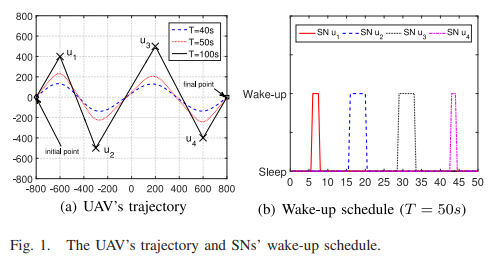
\includegraphics{fig1.png}

    
\end{frame}
\begin{frame}{Comparison of efficiency}
In fig 2, we compare the min-max energy consumption of the SN network with two benchmark cases; static collection where the receiver is at the geometric centre of the SNs, and the case where the UAV flies in a straight line from its initial point to the final point. An idealized lower bound case is also shown, in which we assume that the UAV only collects data when it is on top of each SN and its travel time is ignored. 
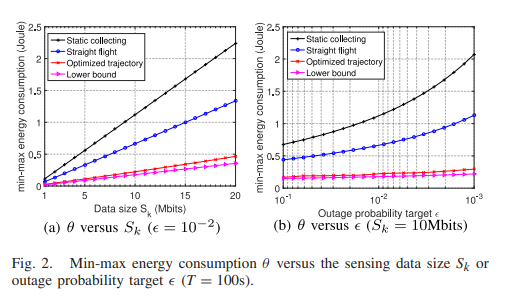
\includegraphics[]{fig2.png}
    
\end{frame}
\begin{frame}{Conclusions}
A novel design has been presented to optimize energy efficiency in UAV enabled WSNs. Using the successive convex optimization technique, an iterative algorithm was constructed to find an efficient sub optimal solution for the trajectory of the UAV and the wake up schedules of each individual SN. The obtained solution is shown to have only a small performance gap compared to the optimal lower bound. 
    
\end{frame}
\end{document}
